\documentclass{article}
\usepackage{graphicx}
\usepackage[margin=2.5cm]{geometry}

\title{Página Web}
\author{Yonhel Mamani Cruz}
\date{May 2025}

\begin{document}

\maketitle

\section{Capturas de Pantalla}

Aquí están las diferentes capturas de pantalla realizadas en Visual Studio Code y los resultados mostrados en la página web del sistema para resolver ecuaciones por el método de Gauss-Jordan.

\begin{figure}[h!]
    \centering
    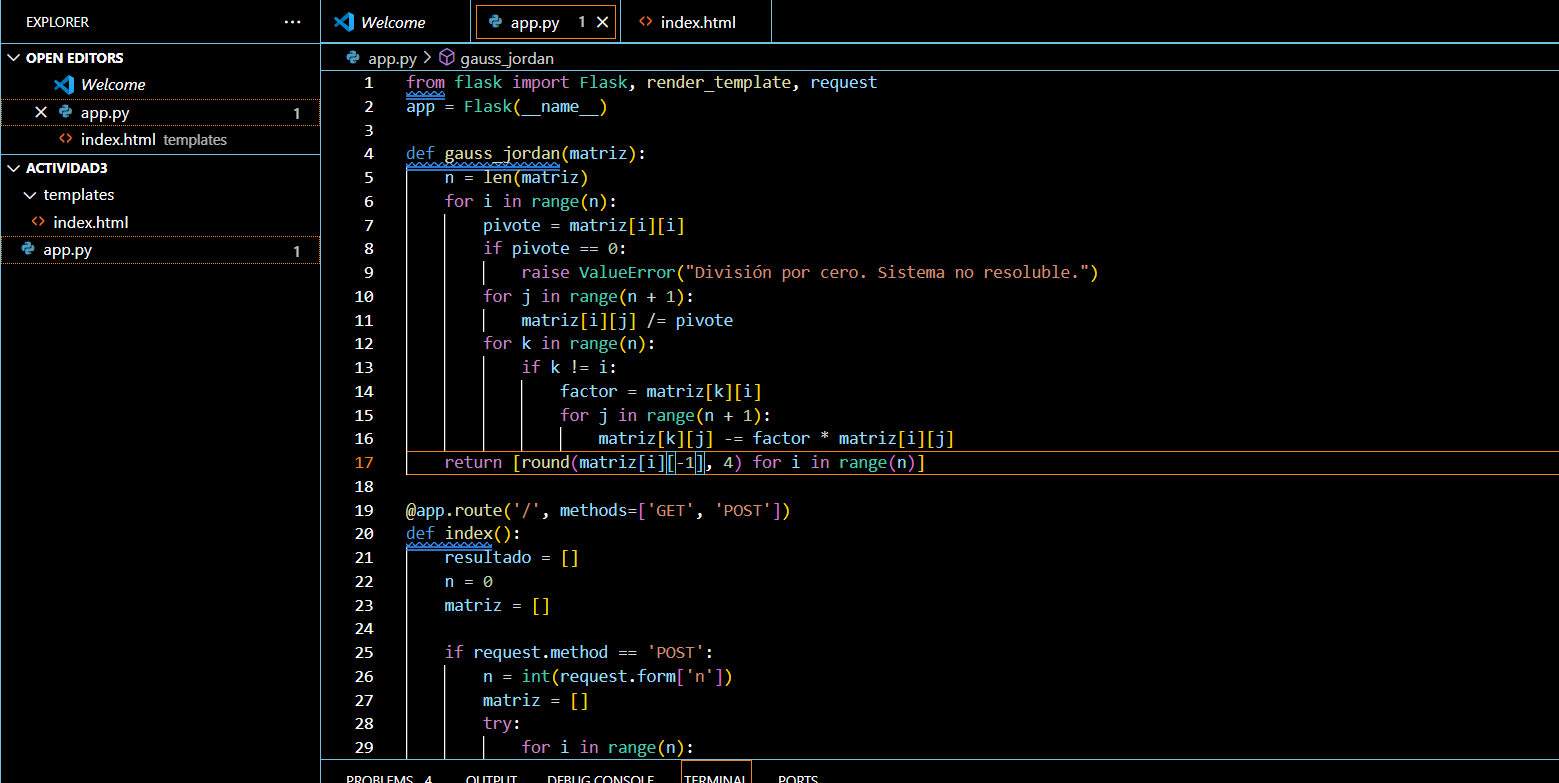
\includegraphics[width=\textwidth]{images/app1.png}
    \caption{app1}
    \label{fig:app1}
\end{figure}

\begin{figure}[h!]
    \centering
    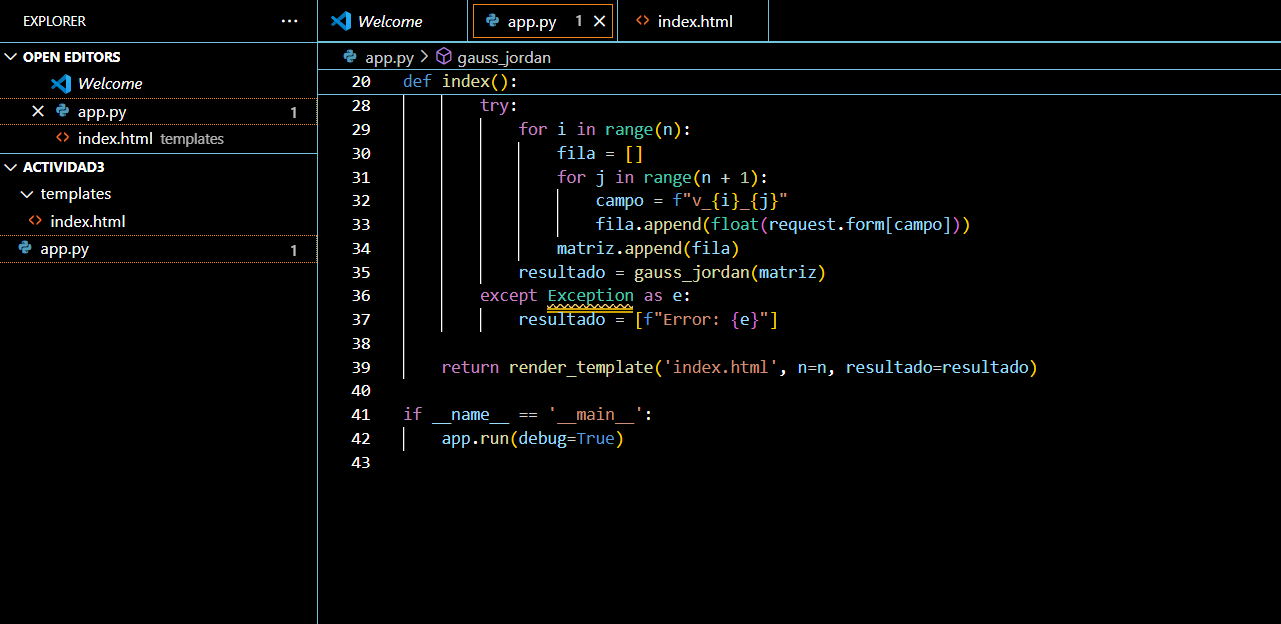
\includegraphics[width=\textwidth]{images/app2.png}
    \caption{app2}
    \label{fig:app2}
\end{figure}

\begin{figure}[h!]
    \centering
    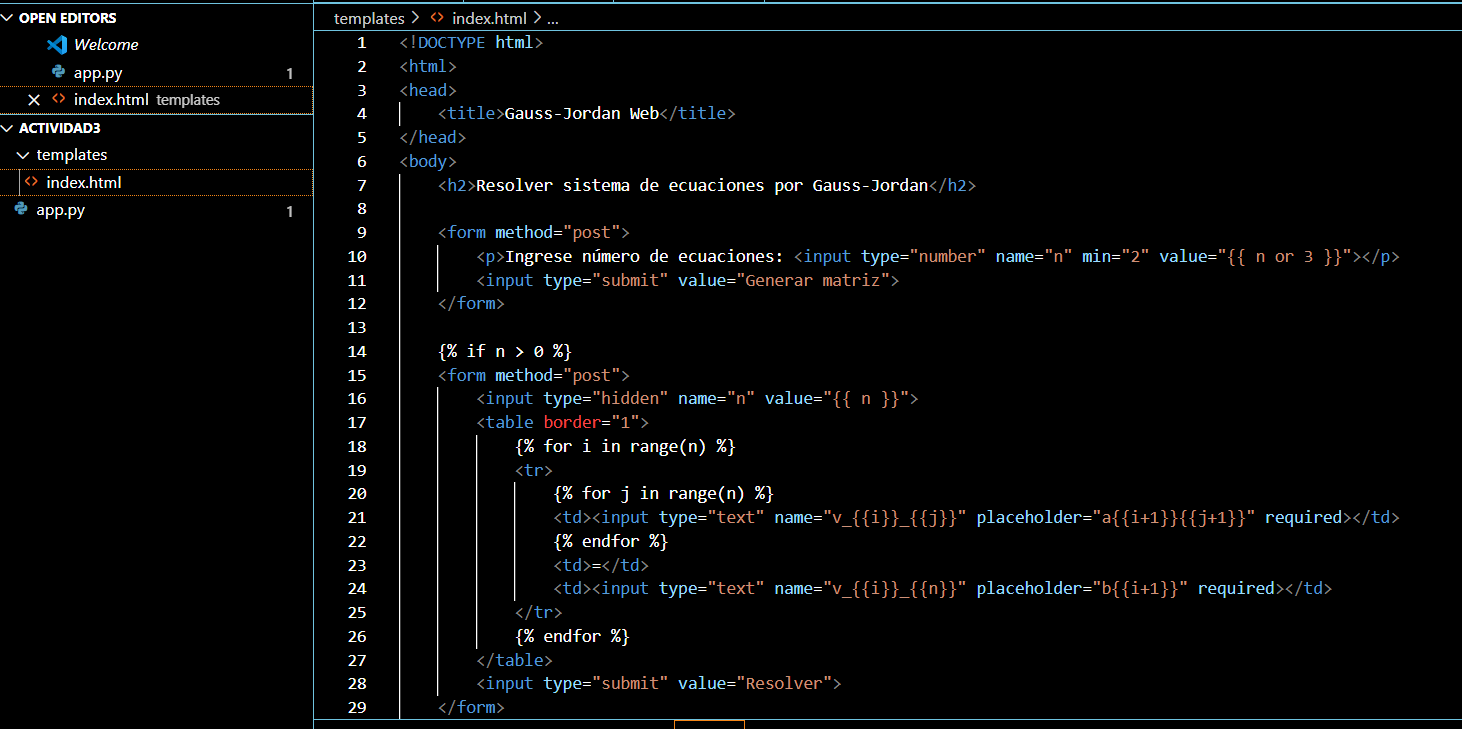
\includegraphics[width=\textwidth]{images/index1.png}
    \caption{index1}
    \label{fig:index1}
\end{figure}

\begin{figure}[h!]
    \centering
    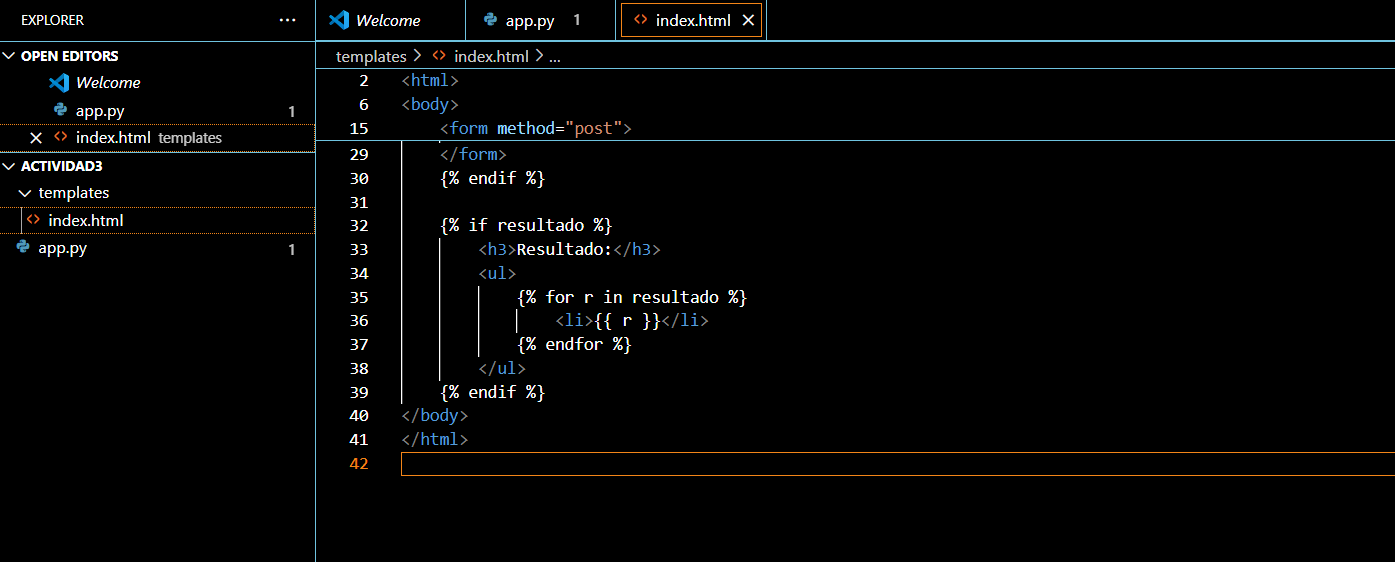
\includegraphics[width=\textwidth]{images/index2.png}
    \caption{index2}
    \label{fig:index2}
\end{figure}

\begin{figure}[h!]
    \centering
    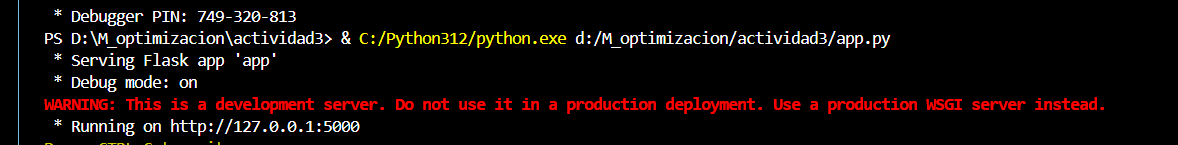
\includegraphics[width=\textwidth]{images/resultadoapp.png}
    \caption{Resultado final del código}
    \label{fig:resultadoapp}
\end{figure}

\begin{figure}[h!]
    \centering
    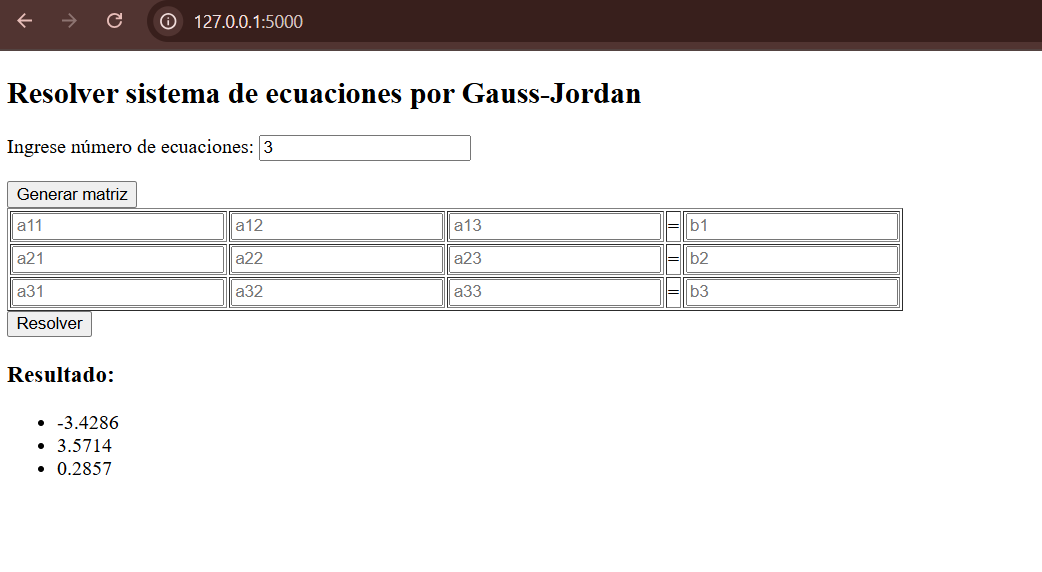
\includegraphics[width=\textwidth]{images/resultado5.png}
    \caption{Resultado final en la página web}
    \label{fig:resultado5}
\end{figure}

\vspace*{10cm} % Ajusta este valor hasta que la conclusión pase a la página 3

\newpage
\vspace*{\fill}
\mbox{} % Página 2


\section*{Conclusión}

Todo este trabajo fue realizado y documentado mediante \LaTeX{}, lo que permitió una presentación clara y profesional.  
Asimismo, este informe y los archivos relacionados han sido organizados y subidos en un repositorio dedicado a \LaTeX{}, facilitando su revisión, colaboración y seguimiento de cambios.


\end{document}




